% Provenance (never printed): see sources/outline_sources.md (Year 1: hotspots and
% mantle plumes; hotspot chains and absolute plate motion; large igneous provinces).
% Hotspot map, pole fit, rates and swell from figdata/bachelor-1/hotspots.py (data
% data/derived/bachelor-1-hotspots.csv, Table 1 of the Morgan and Morgan 2007 electronic
% supplement); exercise and problem values in the Book 3 scratch calculators calc/ch15.py and
% calc/ch15ex.py. "Hotspot" is re-founded from Book 1 (g7 volcanoes), "hotspot track"
% from Book 2 (g11 plate-motions); Book 2 owns the age--distance fit of the Hawaiian
% chain, so this chapter fits the Pacific Euler pole from track directions instead.
\chapter{Puntos calientes y vulcanismo intraplaca}\label{ch:b1:hotspots}

Desde enero de 1983, y durante décadas después, el Kilauea, en la isla de Hawái, entró en erupción casi sin pausa desde un cráter de su
zona de rift oriental, Pu\textquoteleft u~\textquoteleft O\textquoteleft o, vertiendo unos \qty{0.12}{km^3} de lava al año. El Kilauea se alza
en medio de la placa del Pacífico, a miles de kilómetros de cualquier dorsal o fosa. Hacia el noroeste las islas de Hawái son cada vez más
antiguas, luego se hunden bajo el mar y la cadena continúa como una línea de volcanes sumergidos durante miles de kilómetros más. La tectónica
de placas explica los volcanes en las fronteras de placas; este capítulo trata de los que no explica directamente, los \omterm{def:b1:hotspots:hotspot}{puntos calientes}, y de
lo que nos dicen a cambio: cómo se mueven las placas sobre el \omterm{def:b1:layered-earth:layers}{manto} profundo, cuánto calor y roca ascienden desde abajo, y cómo se formaron
unas pocas enormes emisiones de lava, las grandes provincias ígneas.
% ledger: pp1801:kilauea-rate

\begin{recall}
Un \omterm{def:b1:hotspots:hotspot}{punto caliente} alimenta volcanes desde lo profundo del \omterm{def:b1:layered-earth:layers}{manto} mientras la placa se mueve sobre él, y la placa se lleva una \omterm{def:b1:hotspots:track}{traza de punto
caliente} cuyos volcanes son más antiguos con la distancia (libro 1, año 7; libro 2, año 11). Una placa que gira con el \omterm{def:b1:plate-kinematics:euler-pole}{vector de Euler}
$\vec\omega$ se mueve con $\vec v = \vec\omega\times\vec r$, a la velocidad $\omega R\sin\Delta$, perpendicular al \omterm{def:b1:spherical-astronomy:spherical-triangle}{círculo máximo} que la une con
el polo (\cref{ch:b1:plate-kinematics}); el relieve se sostiene por \omterm{def:b1:isostasy-gravity:isostasy}{isostasia} (\cref{ch:b1:isostasy-gravity}); la roca caliente es más ligera en la
fracción $\alpha\,\Delta T$ (\cref{ch:b1:rifts-ridges-margins}).
\end{recall}

\section{Puntos calientes y plumas del manto}\label{sec:b1:hotspots:plumes}

\begin{definition}[Punto caliente]\label{def:b1:hotspots:hotspot}
Un \emph{punto caliente}\index{punto caliente} es una región de vulcanismo cuya posición no depende de las fronteras de placas, activa durante
decenas de millones de años, y que se cree alimentada por \omterm{def:b1:layered-earth:layers}{manto} más caliente que el que lo rodea.
\end{definition}

Cuántos \omterm{def:b1:hotspots:hotspot}{puntos calientes} hay depende de lo que se cuente. La tabla de \omterm{def:b1:hotspots:hotspot}{puntos calientes} usada en este capítulo enumera 68, pero sus autores dejan
fuera varios rasgos que juzgan que no registran el movimiento de una placa, y clasifican como solo probables algunos de los que conservan. Algunos
\omterm{def:b1:hotspots:hotspot}{puntos calientes}, entre ellos Hawái, Islandia y Reunión, tienen trazas largas y regulares y una producción grande, como cabría esperar de una fuente
profunda; otros son pequeños y de vida corta. La mayoría de los volcanes de \omterm{def:b1:hotspots:hotspot}{punto caliente} emiten basalto; donde un \omterm{def:b1:hotspots:hotspot}{punto caliente} yace bajo un
continente, el basalto caliente funde la \omterm{def:b1:layered-earth:layers}{corteza}, y las grandes erupciones se vuelven riolíticas, como en Yellowstone.
% ledger: mm07:table, data:b3-hotspots, yvo:calderas

\begin{definition}[Pluma del manto]\label{def:b1:hotspots:plume}
Una \emph{pluma del manto}\index{pluma del manto} es una columna de roca del \omterm{def:b1:layered-earth:layers}{manto} caliente y boyante que asciende desde una \omterm{def:b1:heat-budget:boundary-layer}{capa límite térmica}
situada en lo profundo del \omterm{def:b1:layered-earth:layers}{manto}. Una pluma nueva tiene una \emph{cabeza} grande y abultada sobre una \emph{cola} larga y estrecha, o conducto; una
vez que la cabeza se ha extendido bajo la \omterm{def:b1:layered-earth:lithosphere}{litosfera}, la cola sigue llevando magma a la superficie durante decenas de millones de años.
\end{definition}

La forma viene del laboratorio. En experimentos en tanque de los años 1970, una capa de fluido ligero y menos viscoso que el fluido que tiene
encima ascendía como una bolsa redonda alimentada por un tubo detrás de ella: un hongo. La cabeza de una \omterm{def:b1:hotspots:plume}{pluma del manto} que llega a la base de la
\omterm{def:b1:layered-earth:lithosphere}{litosfera} se extiende y se aplana; la presión baja, y la roca caliente se funde en grandes cantidades. Los basaltos de inundación encajan en el
cuadro: su vulcanismo dura unos diez millones de años, pero la mayor parte de su volumen se erupciona en un millón de años o menos, y a menudo van
con la ruptura de un continente (\cref{sec:b1:hotspots:lips}).
% ledger: hist:plumes (Whitehead and Luther 1975), cr03:summary

\begin{omfigure}
\begin{tikzpicture}[font=\scriptsize,
  lbl/.style={fill=white, fill opacity=0.8, text opacity=1, inner sep=1pt, align=center}]
% ---- panel (a): the head arrives ----
\begin{scope}
\clip (0,-5) rectangle (6.4,1.3);
\fill[orange!12] (0,-5) rectangle (6.4,0);
\fill[omSea!45] (0,0) rectangle (6.4,0.55);
\fill[omLithBasalt!55] (0,0) rectangle (6.4,-0.9);
% flood basalt: a stack of flat flows on the sea floor
\fill[black!55] (2.5,0) -- (2.7,0.32) -- (6.1,0.32) -- (6.3,0) -- cycle;
\foreach \y in {0.08,0.16,0.24} \draw[white!70!black, line width=0.3pt] (2.62,\y) -- (6.18,\y);
% plume: tail and flattened head
\fill[red!40] (4.25,-5) -- (4.25,-1.7) -- (4.55,-1.7) -- (4.55,-5) -- cycle;
\fill[red!40] (4.4,-1.45) ellipse[x radius=1.9, y radius=0.55];
\draw[red!60!black, line width=0.4pt] (4.25,-5) -- (4.25,-1.95) (4.55,-5) -- (4.55,-1.95);
\draw[red!60!black, line width=0.4pt] (4.4,-1.45) ellipse[x radius=1.9, y radius=0.55];
% melt rising through the plate
\foreach \x in {3.2,3.9,4.6,5.3}
  \draw[red!75!black, line width=0.6pt, decorate, decoration={snake, amplitude=0.6pt, segment length=3pt}] (\x,-1.1) -- (\x,0.05);
\end{scope}
\draw[black!70] (0,-5) rectangle (6.4,1.3);
  \node[lbl, anchor=north west] at (0.1,1.25) {(a) llega la cabeza};
  \node[lbl, anchor=west] at (0.1,-0.45) {litosfera};
  \node[lbl, anchor=west] at (0.1,0.3) {mar};
  \node[lbl, anchor=south] at (4.4,0.62) {basalto de inundación (LIP)};
  \node[lbl, anchor=east] (ph) at (1.9,-1.75) {cabeza de la pluma};
\draw[black!70] (ph.east) -- (2.7,-1.6);
  \node[lbl, anchor=east] at (4.1,-3.6) {cola de la pluma};
  \node[lbl, anchor=west] at (0.1,-4.6) {manto};
% ---- panel (b): the plate has moved on ----
\begin{scope}[xshift=6.8cm]
\begin{scope}
\clip (0,-5) rectangle (6.4,1.3);
\fill[orange!12] (0,-5) rectangle (6.4,0);
\fill[omSea!45] (0,0) rectangle (6.4,0.55);
\fill[omLithBasalt!55] (0,0) rectangle (6.4,-0.9);
% the flood basalt, carried away to the left
\fill[black!55] (-0.9,0) -- (-0.7,0.32) -- (1.0,0.32) -- (1.2,0) -- cycle;
\foreach \y in {0.08,0.16,0.24} \draw[white!70!black, line width=0.3pt] (-0.8,\y) -- (1.08,\y);
% the chain: older volcanoes to the left, lower (they sank as the plate cooled)
\fill[black!35] (1.45,0) -- (1.75,0.2) -- (2.05,0) -- cycle;
\fill[black!38] (2.15,0) -- (2.5,0.3) -- (2.85,0) -- cycle;
\fill[black!42] (2.95,0) -- (3.35,0.42) -- (3.75,0) -- cycle;
\fill[black!65] (3.95,0) -- (4.45,0.95) -- (4.55,0.97) -- (5.05,0) -- cycle;
\fill[red!70!black] (4.43,0.93) -- (4.57,0.95) -- (4.5,1.12) -- cycle;
% the plume tail, still in place, and a small spread of hot rock under the plate
\fill[red!40] (4.35,-5) -- (4.35,-1.1) -- (4.65,-1.1) -- (4.65,-5) -- cycle;
\fill[red!40] (4.5,-1.05) ellipse[x radius=0.75, y radius=0.2];
\draw[red!60!black, line width=0.4pt] (4.35,-5) -- (4.35,-1.2) (4.65,-5) -- (4.65,-1.2);
\draw[red!75!black, line width=0.6pt, decorate, decoration={snake, amplitude=0.6pt, segment length=3pt}] (4.5,-0.95) -- (4.5,0.8);
\end{scope}
\draw[black!70] (0,-5) rectangle (6.4,1.3);
  \node[lbl, anchor=north west] at (0.1,1.25) {(b) mucho después};
  \draw[->, line width=1pt] (3.2,-0.45) -- (1.2,-0.45) node[midway, above=1pt, lbl] {movimiento de la placa};
  \node[lbl, anchor=south] at (0.55,0.38) {el LIP};
  \node[lbl, anchor=south] at (2.7,0.62) {más antiguos, extintos};
  \node[lbl, anchor=west] at (5.0,0.95) {volcán\\activo};
  \node[lbl, anchor=east] at (4.2,-3.6) {cola de la pluma};
  \node[lbl, anchor=west] at (4.75,-2.6) {queda en\\el manto};
\end{scope}
\end{tikzpicture}
\par\smallskip{\small El modelo de pluma de un \omterm{def:b1:hotspots:hotspot}{punto caliente} (esquemático, no a escala). (a)~Una pluma nueva: su cabeza se aplana bajo la
\omterm{def:b1:layered-earth:lithosphere}{litosfera} y se funde al descomprimirse, y un basalto de inundación, una \omterm{def:b1:hotspots:lip}{gran provincia ígnea}, se erupciona en unos pocos millones de años o
menos. (b)~Decenas de millones de años después la placa ha llevado la provincia lejos; la cola estrecha sigue alimentando un volcán activo, y
los volcanes que construyó antes están extintos, más antiguos con la distancia y más bajos, porque se hunden con la placa que se enfría.}
\label{fig:b1:hotspots:plume}
\end{omfigure}

¿Cuál es la evidencia de las plumas? Primero, las propias cadenas con \omterm{def:b1:hotspots:track}{progresión de edad}, que una fuente estrecha fija bajo una placa en
movimiento explica de inmediato (\cref{sec:b1:hotspots:tracks}). Segundo, las lavas de algunos \omterm{def:b1:hotspots:hotspot}{puntos calientes} llevan relaciones inusualmente
altas entre el isótopo ligero y el pesado del helio, interpretadas como la firma de un reservorio profundo que ha conservado parte del gas con el
que se formó la Tierra. Tercero, las fuentes son calientes: las lavas de islas oceánicas y mesetas apuntan a un \omterm{def:b1:layered-earth:layers}{manto} de 200 a \qty{300}{\celsius}
más caliente que el \omterm{def:b1:layered-earth:layers}{manto} bajo las dorsales, cuya temperatura potencial está entre 1280 y \qty{1400}{\celsius}. Cuarto, las imágenes sísmicas del
\omterm{def:b1:layered-earth:layers}{manto}: bajo Hawái, una red de sismómetros en el fondo marino y en las islas captó una columna caliente que desciende hasta el \omterm{def:b1:layered-earth:layers}{manto} inferior, y un
modelo de todo el \omterm{def:b1:layered-earth:layers}{manto} construido en 2015 a partir de formas de onda sísmicas completas muestra columnas amplias, casi verticales, bajo muchos de
los grandes \omterm{def:b1:hotspots:hotspot}{puntos calientes}, que ascienden desde la \omterm{def:b1:layered-earth:discontinuity}{frontera núcleo--manto} hasta unos \qty{1000}{km} bajo la superficie; bajo Hawái, Islandia y
Samoa tienen raíz en parches de velocidad sísmica muy baja en la base del \omterm{def:b1:layered-earth:layers}{manto}. Cómo se hacen estas imágenes pertenece al libro de tercer año universitario.
% ledger: herzberg:tp, wolfe:hawaii, fr15:plumes

Nada de esto es una prueba, y el debate sigue vivo. En la hipótesis de placa, defendida entre otros por Gillian Foulger y James Natland, el vulcanismo
de los \omterm{def:b1:hotspots:hotspot}{puntos calientes} no es especialmente caliente y no necesita una pluma profunda: es un subproducto de la tectónica de placas, alimentado desde
fuentes someras allí donde la \omterm{def:b1:layered-earth:lithosphere}{litosfera} se estira o se fractura. Sus oponentes sostienen que la evidencia de al menos algunas plumas profundas es fuerte,
aunque las imágenes sísmicas aún no son lo bastante nítidas para zanjarlo; y los \omterm{def:b1:hotspots:hotspot}{puntos calientes}, como muestra la sección siguiente, no están del todo fijos.
% ledger: fn03:plate-hypothesis, tarduno:emperor

\section{Trazas de puntos calientes y movimiento de las placas}\label{sec:b1:hotspots:tracks}

\begin{definition}[Traza de punto caliente; progresión de edad]\label{def:b1:hotspots:track}
Una \emph{traza de punto caliente}\index{traza de punto caliente} es la línea de volcanes, montes submarinos y crestas volcánicas que una placa lleva lejos de
un \omterm{def:b1:hotspots:hotspot}{punto caliente} al moverse sobre él. Su \emph{progresión de edad}\index{progresión de edad} es el aumento regular de las edades de sus volcanes con la
distancia al activo. La \emph{dirección} de una traza en el \omterm{def:b1:hotspots:hotspot}{punto caliente} es el \omterm{def:b1:spherical-astronomy:horizontal}{acimut}, medido desde el norte, hacia el que su parte joven se aleja del \omterm{def:b1:hotspots:hotspot}{punto caliente}.
\end{definition}

Si los \omterm{def:b1:hotspots:hotspot}{puntos calientes} se mantienen fijos en el \omterm{def:b1:layered-earth:layers}{manto} profundo, una traza registra el movimiento de la placa sobre el \omterm{def:b1:layered-earth:layers}{manto} profundo: su dirección es la de
la velocidad de la placa en el \omterm{def:b1:hotspots:hotspot}{punto caliente}, y su \omterm{def:b1:hotspots:track}{progresión de edad} da la velocidad. El libro 2, año 11, leyó la velocidad de la placa del Pacífico a partir de
las edades de los volcanes de Hawái. Las direcciones por sí solas dicen ya más: dan el \omterm{def:b1:plate-kinematics:euler-pole}{polo de Euler}.

\begin{proposition}[El polo de Euler a partir de dos trazas]\label{prop:b1:hotspots:two-tracks}
Sea una \omterm{def:b1:plate-kinematics:rigid-plate}{placa rígida} que se mueve sobre dos \omterm{def:b1:hotspots:hotspot}{puntos calientes} fijos en las posiciones $\vec r_1$ y $\vec r_2$, y sean $\vec t_1$ y $\vec t_2$ los vectores
unitarios horizontales a lo largo de sus trazas. Si $\vec t_1$ y $\vec t_2$ no son paralelos, el \omterm{def:b1:plate-kinematics:euler-pole}{vector de Euler} de la placa respecto de los \omterm{def:b1:hotspots:hotspot}{puntos
calientes} es paralelo a $\vec t_1\times\vec t_2$, y su polo es el vector unitario
\[
  \vec p = \pm\frac{\vec t_1\times\vec t_2}{\lVert\vec t_1\times\vec t_2\rVert},
\]
con el signo para el que $(\vec p\times\vec r_1)\cdot\vec t_1 > 0$.
\end{proposition}

\begin{proof}
En cada \omterm{def:b1:hotspots:hotspot}{punto caliente} la placa se mueve con $\vec v_i = \vec\omega\times\vec r_i$ (\cref{thm:b1:plate-kinematics:velocity}), y la traza apunta a lo
largo de ella: $\vec v_i = v_i\vec t_i$ con $v_i > 0$. Un producto vectorial es perpendicular a sus factores, así que $\vec\omega\cdot\vec t_i = 0$ para
$i = 1, 2$: $\vec\omega$ es perpendicular a dos vectores que no son paralelos, luego es paralelo a su producto vectorial. De los dos vectores
unitarios a lo largo de él, el polo es aquel alrededor del cual la rotación es antihoraria, es decir, el que cumple que $\vec p\times\vec r_1$ apunta
en el sentido en que se mueve la placa en el primer \omterm{def:b1:hotspots:hotspot}{punto caliente}, a lo largo de $+\vec t_1$.
\end{proof}

Para usar la proposición se necesitan, en un punto de \omterm{def:b1:spherical-astronomy:geographic}{latitud} $\varphi$ y longitud
$\lambda$, los vectores unitarios hacia el este y el norte,
\[
  \vec e = (-\sin\lambda,\ \cos\lambda,\ 0),\qquad
  \vec n = (-\sin\varphi\cos\lambda,\ -\sin\varphi\sin\lambda,\ \cos\varphi),
\]
en los ejes de \cref{ch:b1:plate-kinematics} ($x$ hacia \ang{0}\,N \ang{0}\,E, $y$ hacia \ang{0}\,N \ang{90}\,E, $z$ hacia el polo norte). Una traza de
\omterm{def:b1:spherical-astronomy:horizontal}{acimut} $\theta$ corre a lo largo de $\vec t = \sin\theta\,\vec e +
\cos\theta\,\vec n$. Con la traza de Hawái, \omterm{def:b1:spherical-astronomy:horizontal}{acimut} \ang{304}, y la traza de Louisville, \omterm{def:b1:spherical-astronomy:horizontal}{acimut} \ang{316}, la proposición sitúa el polo de la placa del
Pacífico en \ang{56.2}\,S, \ang{124.0}\,E (el problema de fin de semana hace el cálculo).
% values (hotspots.py): two_pole_lat -56.1805, two_pole_lon 124.008; ledger: data:b3-hotspots

Dos trazas determinan el polo, pero no lo ponen a prueba. Muchas trazas lo sobredeterminan, y el desajuste dice si los \omterm{def:b1:hotspots:hotspot}{puntos calientes} se comportan
como un marco fijo. W. Jason Morgan, que propuso las plumas profundas, y Jason Phipps Morgan compilaron en 2007 una tabla de 68 \omterm{def:b1:hotspots:hotspot}{puntos calientes}, con,
donde pudieron medirse, la dirección de la traza y la velocidad de la placa sobre el \omterm{def:b1:hotspots:hotspot}{punto caliente}, cada una con su incertidumbre y un peso según su
fiabilidad; un \omterm{def:b1:hotspots:hotspot}{punto caliente} bajo dos placas, como lo está Islandia, tiene una línea para cada una. Quince trazas ponderadas yacen sobre la placa
del Pacífico, trece de ellas con una velocidad.
% ledger: data:b3-hotspots, mm07:table; values (hotspots.py): n_all 71 rows, n_pacific 15, n_rated 13

\begin{method}[Ajuste de un polo de Euler y una velocidad a las trazas de puntos calientes]\label{met:b1:hotspots:pole-fit}
Dados, para $N$ \omterm{def:b1:hotspots:hotspot}{puntos calientes} de una placa, las posiciones, las direcciones de las trazas $\theta_i \pm \sigma_i$ con pesos $w_i$, y para algunos
de ellos las velocidades $v_i$:
\begin{enumerate}
  \item Para un polo de prueba $\vec p$, calcúlese en cada \omterm{def:b1:hotspots:hotspot}{punto caliente} la dirección de $\vec p\times\vec r_i$, el \omterm{def:b1:spherical-astronomy:horizontal}{acimut} $\hat\theta_i$ del
        movimiento que predice (\cref{prop:b1:plate-kinematics:speed}).
  \item Fórmese el desajuste $S(\vec p) = \sum_i w_i\bigl((\hat\theta_i -
        \theta_i)/\sigma_i\bigr)^2$, con cada diferencia llevada entre \ang{-180} y \ang{180}.
  \item Búsquese el polo que minimiza $S$: en una malla de toda la esfera, y luego en una malla más fina alrededor del mejor punto.
  \item Con el polo hallado, calcúlese para cada \omterm{def:b1:hotspots:hotspot}{punto caliente} con velocidad su distancia angular $\Delta_i$ al polo y $x_i = R\sin\Delta_i$. Las
        velocidades deben ser $v_i = \omega x_i$: la velocidad de mínimos cuadrados es
        \[
          \omega = \frac{\sum_i x_i v_i}{\sum_i x_i^2},
        \]
        ya que $\frac{\mathrm d}{\mathrm d\omega}\sum_i (v_i - \omega x_i)^2 =
        -2\sum_i x_i(v_i - \omega x_i)$ se anula allí.
  \item Juzgúese el ajuste: si los \omterm{def:b1:hotspots:hotspot}{puntos calientes} fueran fijos y las incertidumbres honestas, $S$ estaría cerca del número de direcciones menos dos
        (las dos coordenadas del polo ajustado).
\end{enumerate}
\end{method}

Para las quince trazas del Pacífico, el método da el polo \ang{63.8}\,S, \ang{112.5}\,E, a unos \ang{10} del polo de dos trazas, y a partir de las trece
velocidades la velocidad $\omega = \qty{0.92}{\degree\per\Myr}$. En Hawái, a \ang{108.0} del polo, el ajuste predice un movimiento hacia \ang{298} a
\qty{97}{mm.yr^{-1}}; Morgan y Morgan dan $\ang{304}\pm\ang{3}$ y \qty[uncertainty-mode=separate]{92 \pm 3}{mm.yr^{-1}}. El desajuste $S$ es 39, donde
unos \omterm{def:b1:hotspots:hotspot}{puntos calientes} fijos con incertidumbres honestas darían unos 13, y las velocidades se dispersan alrededor de la recta \qty{16}{mm.yr^{-1}}
(valor cuadrático medio): los \omterm{def:b1:hotspots:hotspot}{puntos calientes} del Pacífico forman un marco de referencia bueno a unos pocos grados y a unos pocos centímetros al año,
no mejor.
% values (hotspots.py): pole_lon 112.48, pole_lat -63.78, chi2 38.7829, omega_deg_myr 0.920609,
% hawaii_delta 107.998, hawaii_pred_az 297.656, hawaii_pred_rate 97.3581, rms_rate 15.966;
% angle between the two poles 9.5 deg (calc/ch15.py); ledger: data:b3-hotspots

La prueba más conocida del marco fijo es la curva de la cadena Hawái--Emperador. La rama hawaiana corre hacia el noroeste; los montes submarinos
Emperador corren casi hacia el norte, hasta el monte Meiji, de más de 81 millones de años, que está a punto de hundirse en la confluencia de las fosas
de Kuriles--Kamchatka y de las Aleutianas. ¿Fue la curva un cambio en el movimiento de la placa? La imantación de las lavas del Emperador, medida en
testigos perforados en los montes submarinos, registra la \omterm{def:b1:spherical-astronomy:geographic}{latitud} a la que se enfrió cada una (el método pertenece al libro de tercer año universitario):
se formaron más al norte de donde está hoy Hawái, y entre 81 y 47 millones de años atrás el propio \omterm{def:b1:hotspots:hotspot}{punto caliente} se desplazó hacia el sur a más de
\qty{40}{mm} al año. Gran parte de la cadena Emperador registra el \omterm{def:b1:hotspots:hotspot}{punto caliente}, no la placa. Sin embargo, la placa también cambió: nuevas edades sitúan
el comienzo de la curva cerca del monte Kimmei, hace unos 50 millones de años, cuando se realinearon las dorsales de expansión del Pacífico. La pluma puede
incluso ser más antigua que la cadena: se cree que la cabeza que la alimentó primero formó una meseta hace unos 100 millones de años, que se hundió en una
fosa hace 20 a 30 millones de años y que yace hoy a unos \qty{810}{km} de profundidad bajo Siberia, al oeste del mar de Ojotsk.
% ledger: tarduno:emperor, sharp:bend, wei:plume-head

\begin{omfigure}
\begin{tikzpicture}
\begin{axis}[omrecord, width=0.78\linewidth, height=6.2cm, xmin=0, xmax=7000, ymin=0, ymax=160,
  xlabel={$R\sin\Delta$, distancia al eje de rotación (\unit{km})},
  ylabel={velocidad sobre el punto caliente (\unit{mm.yr^{-1}})},
  xticklabel style={/pgf/number format/set thousands separator={}},
  legend style={font=\scriptsize, at={(0.03,0.97)}, anchor=north west, cells={anchor=west}}]
% computed in figdata/bachelor-1/hotspots.py; ledger: data:b3-hotspots; values: omega_deg_myr 0.920609
\addplot[only marks, mark=*, mark size=1.5pt, omDef, error bars/.cd, y dir=both, y explicit]
  table[x=x, y=rate, y error=srate] {figdata/out/bachelor-1-hotspots-rates.dat};
\addlegendentry{puntos calientes del Pacífico}
\addplot[black, densely dashed, line width=0.7pt] table[x=x, y=rate] {figdata/out/bachelor-1-hotspots-rates-fit.dat};
\addlegendentry{$\omega R\sin\Delta$, $\omega = \ang{0.92}$ por millón de años}
\draw[black!60] (axis cs:6060,90) -- (axis cs:6550,55) node[font=\scriptsize, anchor=north, black] {Hawái};
\node[font=\scriptsize, anchor=north west] at (axis cs:4880,64) {Louisville};
\node[font=\scriptsize, anchor=west] at (axis cs:3960,43) {Cobb};
\node[font=\scriptsize, anchor=east] at (axis cs:3570,40) {Bowie};
\end{axis}
\end{tikzpicture}
\par\smallskip{\small Las velocidades de la placa del Pacífico sobre trece de sus \omterm{def:b1:hotspots:hotspot}{puntos calientes}, con sus incertidumbres, frente a la distancia
de cada \omterm{def:b1:hotspots:hotspot}{punto caliente} al eje de rotación del polo ajustado. Una \omterm{def:b1:plate-kinematics:rigid-plate}{placa rígida} que gira alrededor de ese polo las pone sobre una recta que pasa por el
origen; la recta de mínimos cuadrados da $\omega = \qty{0.92}{\degree\per\Myr}$. La mayoría de los \omterm{def:b1:hotspots:hotspot}{puntos calientes} yacen a 6000 a \qty{6400}{km} del
eje, donde la velocidad es casi la misma; la dispersión allí, mayor que las barras de error, muestra los límites de un marco fijo. Datos: W.~J. y
J.~P. Morgan (2007), Tabla~1 de su suplemento electrónico.}
\label{fig:b1:hotspots:rates}
\end{omfigure}

\begin{omfigure}
\begin{tikzpicture}
\begin{axis}[ommap, width=0.96\linewidth, xtick={-180,-90,...,180}, ytick={-60,0,60},
  legend style={font=\scriptsize, at={(0.01,0.02)}, anchor=south west, cells={anchor=west}}]
% computed in figdata/bachelor-1/hotspots.py; ledger: data:b3-hotspots, data:ne-land, data:pb2002
\addplot[fill=omLithAlluv, draw=black!45, line width=0.2pt, forget plot] table {figdata/out/shared-geo-land.dat};
\addplot[omRidge, line width=0.5pt, forget plot] table {figdata/out/shared-geo-ridge.dat};
\addplot[omRidge!70!black, line width=0.5pt, forget plot] table {figdata/out/shared-geo-transform.dat};
\addplot[omTrench, line width=0.5pt, forget plot] table {figdata/out/shared-geo-subduction.dat};
\addplot[black!65, line width=0.5pt, forget plot] table {figdata/out/shared-geo-collision.dat};
\addplot[black, line width=0.7pt, -{Stealth[length=3.5pt]}, quiver={u=\thisrow{dx}, v=\thisrow{dy}}, forget plot]
  table[x=lon, y=lat] {figdata/out/bachelor-1-hotspots-map-arrows.dat};
\addplot[only marks, mark=*, mark size=1.3pt, draw=black, fill=orange!90!red] table {figdata/out/bachelor-1-hotspots-map-hs.dat};
\addlegendentry{punto caliente}
\addplot[only marks, mark=star, mark size=3.2pt, line width=0.8pt, omDef] table {figdata/out/bachelor-1-hotspots-map-pole.dat};
\addlegendentry{polo de Euler de la placa del Pacífico}
\draw[black, line width=0.7pt, -{Stealth[length=3.5pt]}] (axis cs:-40,-80) -- (axis cs:-25,-80);
\node[font=\scriptsize, anchor=west, fill=white, fill opacity=0.75, text opacity=1, inner sep=1pt]
  at (axis cs:-23,-80) {\qty{10}{cm} al año};
\node[font=\scriptsize, anchor=north, fill=white, fill opacity=0.75, text opacity=1, inner sep=1pt] at (axis cs:-150,16) {Hawái};
\node[font=\scriptsize, anchor=north, fill=white, fill opacity=0.75, text opacity=1, inner sep=1pt] at (axis cs:-140.6,-56) {Louisville};
\node[font=\scriptsize, anchor=south, fill=white, fill opacity=0.75, text opacity=1, inner sep=1pt] at (axis cs:-100,49) {Yellowstone};
\node[font=\scriptsize, anchor=south, fill=white, fill opacity=0.75, text opacity=1, inner sep=1pt] at (axis cs:-17.3,66) {Islandia};
\node[font=\scriptsize, anchor=north, fill=white, fill opacity=0.75, text opacity=1, inner sep=1pt] at (axis cs:55.7,-23.5) {Reunión};
\end{axis}
\end{tikzpicture}
\par\smallskip{\small Los 68 \omterm{def:b1:hotspots:hotspot}{puntos calientes} de W.~J. y J.~P. Morgan (2007). Flechas: el movimiento de la placa sobre cada \omterm{def:b1:hotspots:hotspot}{punto caliente} donde se
midió, a lo largo de la dirección de la traza y con una longitud proporcional a la velocidad (escala abajo, al sur del Atlántico); donde un \omterm{def:b1:hotspots:hotspot}{punto
caliente} yace bajo dos placas, como Islandia, se dibujan ambas. La estrella es el \omterm{def:b1:plate-kinematics:euler-pole}{polo de Euler} de la placa del Pacífico respecto de los \omterm{def:b1:hotspots:hotspot}{puntos
calientes}, ajustado a las quince trazas del Pacífico mediante \cref{met:b1:hotspots:pole-fit}: las flechas del Pacífico giran alrededor de él. Fronteras
de placas: PB2002 (rojo: dorsales; rojo oscuro: transformantes; azul: zonas de subducción; gris: zonas de colisión).}
\label{fig:b1:hotspots:map}
\end{omfigure}


Las \omterm{def:b1:hotspots:track}{trazas de puntos calientes} también cruzan continentes. Mientras la placa norteamericana se desplazaba hacia el suroeste sobre el \omterm{def:b1:hotspots:hotspot}{punto caliente} de
Yellowstone, se formó una cadena de grandes calderas, cada vez más antiguas hacia el suroeste a lo largo de la llanura del río Snake. En su extremo
lejano, en la frontera de Nevada y Oregón, la caldera de McDermitt, de unos \qty{40}{km} de ancho, se hundió hace 16.4 millones de años en una erupción
de unos \qty{1000}{km^3}. En el propio Yellowstone, la primera de tres erupciones formadoras de caldera, hace 2.1 millones de años, liberó unos
\qty{2400}{km^3} de magma y dejó una caldera de más de \qty{100}{km} de ancho; la última, hace 640\,000 años, dio la caldera actual de Yellowstone, de
\qty{55}{km} por 80. Desde hace 10 millones de años el inicio de las erupciones de caldera se ha desplazado hacia el noreste a
$\qty[uncertainty-mode=separate]{2.9 \pm 0.5}{cm}$ al año, y Morgan y Morgan dan a la placa una velocidad de
\qty[uncertainty-mode=separate]{26 \pm 5}{mm.yr^{-1}} sobre el \omterm{def:b1:hotspots:hotspot}{punto caliente}, hacia \ang{235}; las calderas más antiguas, como muestra
\cref{exo:b1:hotspots:8}, se movieron más deprisa.
% ledger: henry:mcdermitt, yvo:calderas, pm90:track, data:b3-hotspots

\section{Abultamientos, flotabilidad y suministro de magma}\label{sec:b1:hotspots:swells}

Hawái no se alza sobre fondo oceánico ordinario. En 1953 Robert Dietz y William Menard describieron la amplia elevación del fondo marino sobre la que
se asientan las islas, el abultamiento hawaiano. El abultamiento no está compensado por \omterm{def:b1:layered-earth:layers}{corteza} gruesa: lo sostiene desde abajo la roca caliente y ligera
de la pluma a medida que se extiende bajo la placa, un soporte \emph{dinámico}. Sobre el abultamiento el \omterm{def:b1:heat-budget:heat-flow}{flujo de calor} en superficie es como mucho de 5 a
\qty{10}{mW.m^{-2}} más alto que alrededor, y quizá no más alto en absoluto.
% ledger: hist:plumes (Dietz and Menard 1953), vh89:swell-heat

Su forma puede leerse en la malla global de profundidades. Tómense secciones a través de la traza, perpendiculares a su dirección, cada
\qty{50}{km} desde el \omterm{def:b1:hotspots:hotspot}{punto caliente} hasta \qty{1000}{km} aguas abajo; a cada distancia del eje de la cadena, la mediana de las profundidades en estas
secciones da un perfil que conserva el abultamiento y suaviza los volcanes aislados (la figura tras la siguiente proposición). Lejos de la cadena, de
\qty{1000}{km} a \qty{1500}{km} a cada lado, el fondo yace a \qty{5274}{m}. Cerca de ella, las islas y los montes submarinos se alzan hasta \qty{3}{km} más
alto; sustitúyanse por una recta a través de los \qty{300}{km} de la cadena, y lo que queda es el abultamiento: de unos \qty{690}{m} de altura como mucho,
de unos cientos de kilómetros de ancho a cada lado, con una sección de $A \approx \qty{4.8e8}{m^2}$ sobre el fondo lejano.
% values (hotspots.py): swell_ref -5273.64, swell_height 690.636, swell_area_m2 4.82786e8;
% ledger: data:etopo1, data:b3-hotspots (Hawaii 19.0 N 155.2 W, track 304)

El abultamiento mide la pluma. Se lleva con la placa y se rehace sobre el \omterm{def:b1:hotspots:hotspot}{punto caliente}, así que la pluma debe suministrar flotabilidad tan deprisa
como la placa se la lleva.

\begin{proposition}[Flujo de flotabilidad de una pluma]\label{prop:b1:hotspots:buoyancy}
Sea una placa que se mueve a la velocidad $v$ sobre un \omterm{def:b1:hotspots:hotspot}{punto caliente}, y sea el abultamiento alrededor de la traza de sección $A$ sobre el fondo lejos
de él, estando el abultamiento en equilibrio isostático (\cref{def:b1:isostasy-gravity:isostasy}) y sostenido por roca ligera que se lleva junto con la
placa. Entonces la pluma aporta un déficit de masa, su \emph{flujo de flotabilidad}, a razón de
\[
  B = (\rho_m - \rho_w)\,A\,v ,
\]
donde $\rho_m$ es la densidad del \omterm{def:b1:layered-earth:layers}{manto} y $\rho_w$ la del agua de mar.
\end{proposition}

\begin{proof}
Considérese una columna a través del abultamiento, donde el fondo está elevado $h$, y una columna lejos de él, ambas hasta una \omterm{def:b1:isostasy-gravity:isostasy}{profundidad de
compensación}. Entre los dos fondos, la columna lejana tiene agua y la columna del abultamiento roca: la columna del abultamiento tiene la masa en
exceso $(\rho_m - \rho_w)h$ por unidad de área allí. Masas iguales por encima de la \omterm{def:b1:isostasy-gravity:isostasy}{profundidad de compensación}
(\cref{prop:b1:isostasy-gravity:equal-mass}) exigen un déficit de masa del mismo tamaño más abajo en la columna del abultamiento, en la roca ligera de la
pluma. A lo largo de la traza, el déficit por unidad de longitud de traza es $\int(\rho_m - \rho_w)h\,\mathrm dy = (\rho_m - \rho_w)A$. En un tiempo
$\mathrm dt$ la placa lleva una longitud $v\,\mathrm dt$ de abultamiento aguas abajo, con su déficit, y el abultamiento sobre el \omterm{def:b1:hotspots:hotspot}{punto caliente} conserva
su forma: la pluma debe suministrar el déficit $(\rho_m - \rho_w)A\,v\,\mathrm dt$.
\end{proof}

\begin{omfigure}
\begin{tikzpicture}
\begin{axis}[omrecord, width=0.86\linewidth, height=6cm, xmin=-1500, xmax=1500, xtick={-1500,-1000,...,1500}, ymin=-6000, ymax=-1000,
  xlabel={distancia a través de la cadena de Hawái, del suroeste al noreste (\unit{km})},
  ylabel={profundidad del fondo marino (\unit{m})},
  xticklabel style={/pgf/number format/set thousands separator={}},
  yticklabel style={/pgf/number format/set thousands separator={}},
  legend style={font=\scriptsize, at={(0.99,0.97)}, anchor=north east, cells={anchor=west}}]
% computed in figdata/bachelor-1/hotspots.py; ledger: data:etopo1, data:b3-hotspots
\addplot[name path=hi, draw=none, forget plot] table[x=d, y=q75] {figdata/out/bachelor-1-hotspots-swell.dat};
\addplot[name path=lo, draw=none, forget plot] table[x=d, y=q25] {figdata/out/bachelor-1-hotspots-swell.dat};
\addplot[omSea!60, forget plot] fill between[of=hi and lo];
\addplot[black, line width=0.8pt] table[x=d, y=med] {figdata/out/bachelor-1-hotspots-swell.dat};
\addlegendentry{profundidad mediana}
\addplot[omDef, line width=0.9pt, densely dashed] table[x=d, y=swell] {figdata/out/bachelor-1-hotspots-swell-ref.dat};
\addlegendentry{abultamiento, sin la cadena}
\addplot[black!60, densely dotted, line width=0.7pt] table[x=d, y=ref] {figdata/out/bachelor-1-hotspots-swell-ref.dat};
\addlegendentry{referencia, de 1000 a \qty{1500}{km} fuera}
\node[font=\scriptsize, anchor=south] at (axis cs:-330,-3300) {la cadena};
\end{axis}
\end{tikzpicture}
\par\smallskip{\small El abultamiento hawaiano. Cada punto es la mediana de 21 profundidades, tomadas en secciones a través de la cadena cada
\qty{50}{km} desde el \omterm{def:b1:hotspots:hotspot}{punto caliente} hasta \qty{1000}{km} aguas abajo, a la misma distancia del eje de la cadena; la banda sombreada contiene la
mitad central de las 21 profundidades. La cadena misma, un pico estrecho, se sustituye por una recta (discontinua) para dejar el abultamiento, de
unos \qty{690}{m} sobre el fondo lejos de la cadena (de puntos). Profundidades: ETOPO1, muestreado a un grado.}
\label{fig:b1:hotspots:swell}
\end{omfigure}

Un flujo de flotabilidad es un flujo de masa faltante: cuenta cuán deprisa la pluma sube roca ligera. Lo que hace ligera la roca es el calor, así que
el flujo de flotabilidad es también un \omterm{def:b1:heat-budget:heat-flow}{flujo de calor}.

\begin{proposition}[Calor transportado por una pluma]\label{prop:b1:hotspots:heat}
Si la roca de una pluma está $\Delta T$ más caliente que el \omterm{def:b1:layered-earth:layers}{manto} que la rodea, con el coeficiente de dilatación térmica $\alpha$ y el calor
específico $c_p$, su flujo de flotabilidad $B$ y el calor en exceso que transporta, $Q$, satisfacen
\[
  Q = \frac{c_p}{\alpha}\,B ,
\]
cualquiera que sea $\Delta T$.
\end{proposition}

\begin{proof}
Sea la pluma la que lleva la masa $\Phi$ de roca caliente por unidad de tiempo. Cada unidad de volumen es más ligera que el \omterm{def:b1:layered-earth:layers}{manto} en
$\rho_m\alpha\,\Delta T$, lo que es, en primer orden, un déficit de masa $\alpha\,\Delta T$ por unidad de masa: $B =
\alpha\,\Delta T\,\Phi$. Cada
unidad de masa lleva el calor en exceso $c_p\,\Delta T$: $Q = c_p\,\Delta T\,\Phi$. Dividiendo, $\Delta T$ y $\Phi$ se cancelan.
\end{proof}

Para Hawái, con $\rho_m - \rho_w = \qty{2300}{kg.m^{-3}}$, $A =
\qty{4.83e8}{m^2}$ y $v = \qty{92}{mm.yr^{-1}} = \qty{2.92e-9}{m.s^{-1}}$,
\[
  B = 2300\times\num{4.83e8}\times\num{2.92e-9} \approx \qty{3240}{kg.s^{-1}}:
\]
la pluma aporta unas tres toneladas de masa faltante cada segundo. Las rocas almacenan de 2 a \qty{3}{MJ} por metro cúbico y por kelvin; con
\qty{3}{MJ}, el \omterm{def:b1:layered-earth:layers}{manto}, de densidad \qty{3300}{kg.m^{-3}}, tiene
$c_p \approx \qty{910}{J.kg^{-1}.K^{-1}}$;
con $\alpha = \qty{3.2e-5}{K^{-1}}$,
\[
  Q = \frac{910}{\num{3.2e-5}}\times3240 \approx \qty{9.2e10}{W},
\]
\qty{0.2}{\percent} de los \qty{47}{TW} que salen de toda la Tierra. La pluma más fuerte de la Tierra es un elemento pequeño en el balance térmico
del planeta (\cref{ch:b1:heat-budget}); la mayor parte del calor sale a través del fondo oceánico formado en las dorsales.
% values (hotspots.py): swell_B_kg_s 3237.18; Q = 9.1951e10 W (calc/ch15.py);
% ledger: data:b3-hotspots (92 mm/yr), delaney86:properties (Book 2 row), parsons:plate-model (alpha), dd10:total

El magma cuenta la misma historia. Desde hace 81 millones de años el \omterm{def:b1:hotspots:hotspot}{punto caliente} ha construido la cadena Hawái--Emperador, unos dos millones de
kilómetros cúbicos de basalto una vez contado el hundimiento de la placa bajo su carga, un promedio de \qty{0.025}{km^3} al año; pero cerca de un
cuarto de ello se erupcionó en los últimos seis millones de años, y el Kilauea solo recibe hoy unos \qty{0.1}{km^3} de magma al año. El Mauna Loa, el
mayor volcán de las islas, contiene unos \qty{74000}{km^3}, y el Mauna Kea, su vecino, se alza \qty{4205}{m} sobre el mar. Sin embargo, las dorsales
producen unos \qty{21}{km^3} de \omterm{def:b1:rifts-ridges-margins:oceanic-crust}{corteza oceánica} al año, doscientas veces el suministro actual del Kilauea.
% ledger: pp1801:chain-volume, pp1801:kilauea-supply, pp1801:volumes, data:pb2002 (ridge_budget.py 21.36 km3/yr)

\begin{omfigure}
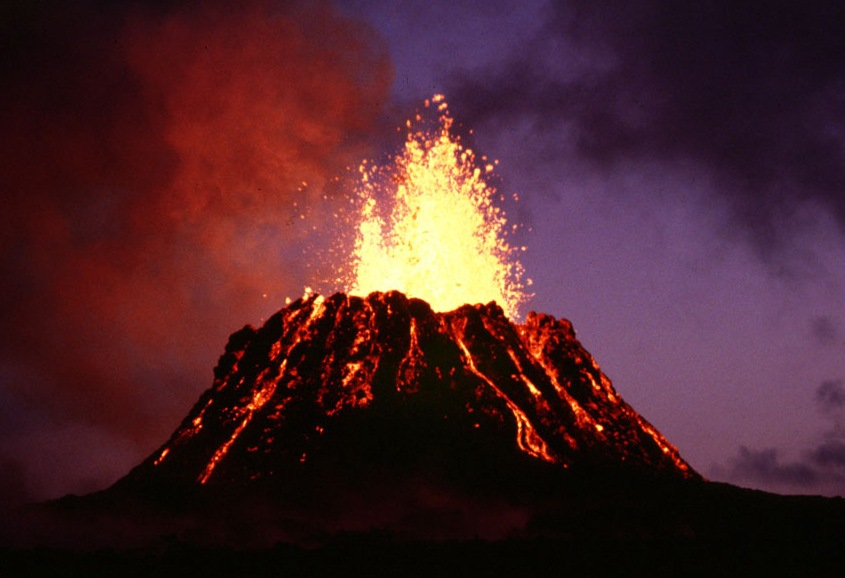
\includegraphics[width=0.55\linewidth]{images/book3/b1-puu-oo-1983.jpg}
\par\smallskip{\small Una fuente de lava en el cono Pu\textquoteleft
u~\textquoteleft O\textquoteleft o, en la zona de rift oriental del Kilauea, el 29 de junio de 1983, en el primer año de una erupción que duró décadas:
lava basáltica, caliente y fluida, lanzada en un chorro y que cae de nuevo alrededor del cráter. Fotografía: G.~E.~Ulrich, U.S. Geological Survey,
dominio público (Wikimedia Commons).}
\label{fig:b1:hotspots:puu-oo}
\end{omfigure}
% ledger: commons:puu-oo, pp1801:kilauea-rate

\begin{history}[Un marco fijo para las placas]
En 1963 John Tuzo Wilson explicó las islas hawaianas, cada vez más antiguas a lo largo de una línea, por una fuente de lava mantenida en el núcleo
lento de una celda de convección del \omterm{def:b1:layered-earth:layers}{manto}, mientras que la parte superior más rápida de la celda llevaba el fondo oceánico sobre ella. En 1971 y 1972
W. Jason Morgan convirtió esa fuente en una pluma, de unos \qty{150}{km} de ancho, que asciende desde la parte más baja del \omterm{def:b1:layered-earth:layers}{manto} y así casi fija
mientras las placas se mueven sobre ella; los experimentos en tanque pronto mostraron cómo se ve una pluma así. Los \omterm{def:b1:hotspots:hotspot}{puntos calientes} se volvieron un
marco en el que las placas podían medirse frente al \omterm{def:b1:layered-earth:layers}{manto}, no solo unas frente a otras. Medio siglo después se sabe que el marco se desplaza, el \omterm{def:b1:hotspots:hotspot}{punto
caliente} hawaiano entre otros, pero con la lentitud suficiente para que las trazas del Pacífico sigan dando el movimiento de la placa sobre el \omterm{def:b1:layered-earth:layers}{manto} con
unos pocos grados y unos pocos centímetros al año, como mostró el ajuste de este capítulo.
\end{history}
% ledger: hist:plumes, tarduno:emperor

\section{Grandes provincias ígneas}\label{sec:b1:hotspots:lips}

\begin{definition}[Gran provincia ígnea]\label{def:b1:hotspots:lip}
Una \emph{gran provincia ígnea}\index{gran provincia ígnea} (LIP) es una acumulación de roca ígnea, en su mayor parte basalto, que no se forma por la
expansión ordinaria en una dorsal, cubre más de \qty{e5}{km^2}, contiene más de \qty{e5}{km^3} y se emplazó en como máximo unos 50 millones de años, la mayor
parte en pulsos de 1 a 5 millones de años que llevan más de tres cuartos de su volumen. En tierra las LIP son sobre todo basaltos de inundación; en los
océanos, mesetas oceánicas.
\end{definition}

Un LIP típico cubre cerca de un millón de kilómetros cuadrados y contiene cerca de un millón de kilómetros cúbicos de lava, la mayor parte erupcionada
en un millón de años o menos. Sus lavas se apilan en coladas casi planas, que la erosión corta en escalones, los \emph{traps} que dan nombre a estas
provincias. La tabla enumera las principales de los últimos 260 millones de años.
% ledger: be08:definition, cr03:summary

\begin{omfigure}
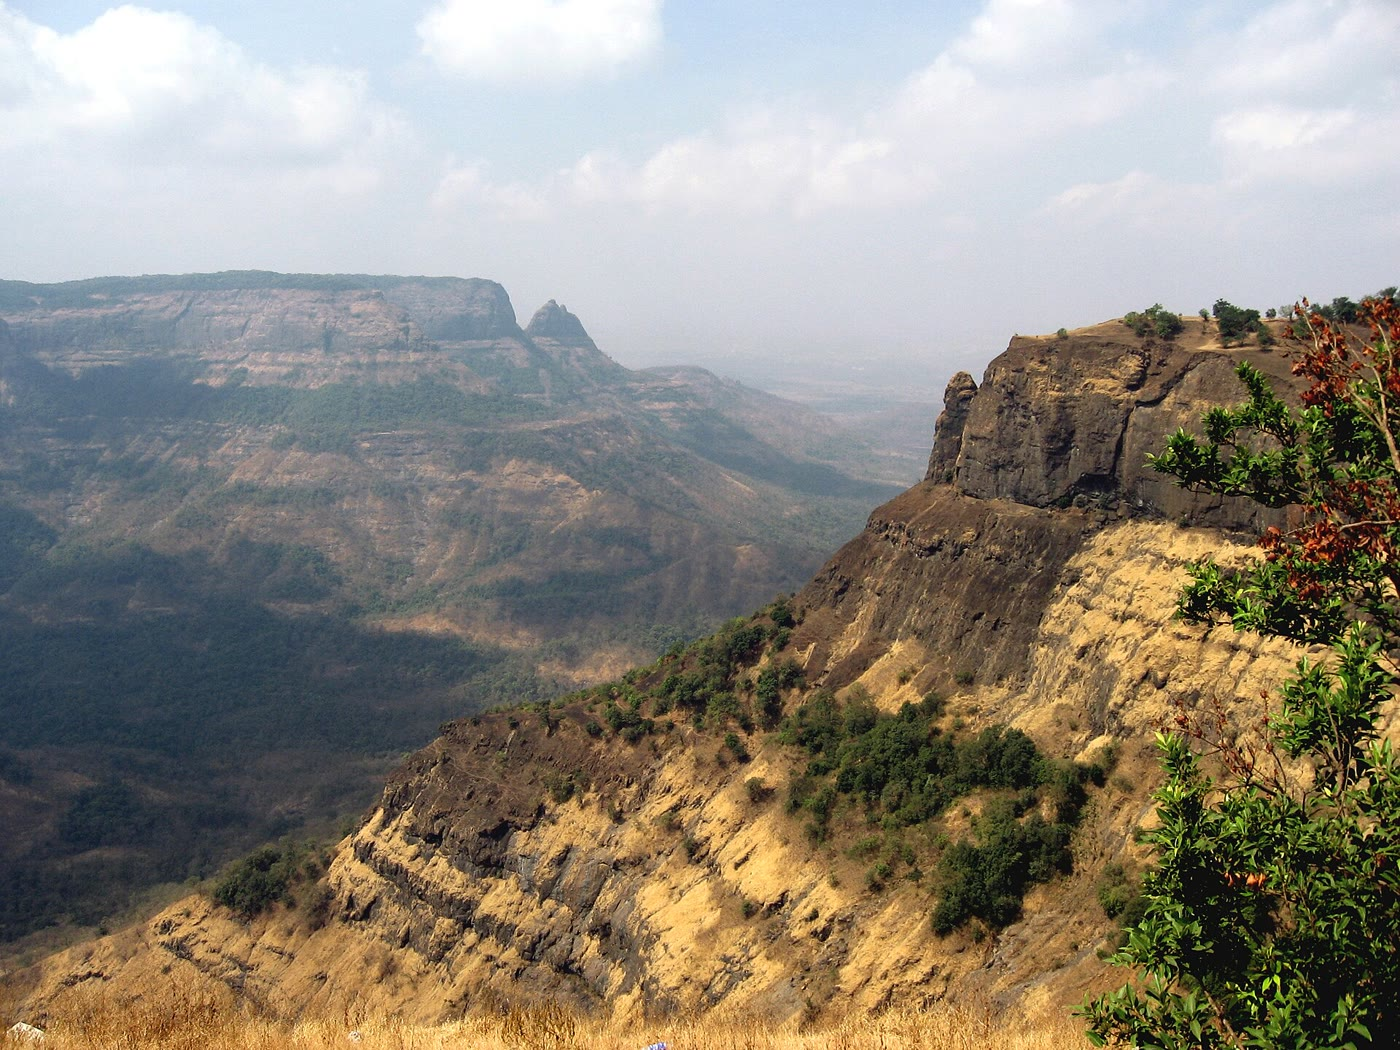
\includegraphics[width=0.55\linewidth]{images/book3/b1-deccan-matheran.jpg}
\par\smallskip{\small Los Ghats Occidentales cerca de Matheran, India: colinas de cima plana talladas en una pila de coladas de lava casi horizontales
de los Deccan Traps, cuyas capas resistentes forman los escalones de las laderas. Fotografía: Nicholas (Nichalp), CC BY-SA 2.5 (Wikimedia Commons).}
\label{fig:b1:hotspots:deccan}
\end{omfigure}
% ledger: commons:matheran

\begin{center}
\small
\begin{tabular}{llll}
\hline
provincia & edad (Ma) & área (\unit{Mkm^2}) & primer volumen (\unit{Mkm^3})\\
\hline
Columbia River & 16 & 0.2 & 0.2\\
Etiopía--Yemen & 30 & 0.7 & 1.2\\
Atlántico Norte & 61 y 56 & 1.2 & más de 2\\
Deccan & 65.5 & 0.5 (una vez 1.8) & de 2 a 4\\
Ontong Java & 122 y 90 & 2 & 44 (\omterm{def:b1:layered-earth:layers}{corteza} entera)\\
Paraná--Etendeka & 133 & 1.5 (una vez más de 2) & más de 2.3\\
Karoo--Ferrar & 183 & 3.1 & más de 2.5\\
Atlántico Central (CAMP) & 201 & una vez hasta 7 & más de 2\\
Traps siberianos & 250 & 0.4 (una vez más de 4) & más de 3\\
Emeishan & 259 & 0.5 (una vez de 2 a 5) & más de 1\\
\hline
\end{tabular}
\par\smallskip{\small Edades medias; áreas tal como son hoy, y como se erupcionaron donde existe una estimación; volúmenes de lava tal como se
erupcionaron en primer lugar, excepto para la meseta de Ontong Java, cuya cifra cuenta toda su \omterm{def:b1:layered-earth:layers}{corteza} engrosada. Datos: V.~Courtillot y
P.~Renne (2003).}
\end{center}
% ledger: cr03:table

\noindent El modelo de pluma esbozado en \cref{sec:b1:hotspots:plumes} explica tanto el tamaño como la prisa: una cabeza de pluma de cientos de
kilómetros de ancho llega a la base de la \omterm{def:b1:layered-earth:lithosphere}{litosfera}, se descomprime y se funde, e inunda la superficie; después la cola sigue construyendo una traza
ordinaria de \omterm{def:b1:hotspots:hotspot}{punto caliente}. Se cree que varias provincias yacen en el extremo antiguo de una traza viva: las trampas del Deccan y el \omterm{def:b1:hotspots:hotspot}{punto caliente}
de Reunión, Paraná--Etendeka y Tristán da Cunha, unidas por la dorsal de Walvis, y los basaltos del Columbia River y Yellowstone.
% ledger: cr03:deccan (Reunion hot spot, plume-head model), be08:ojmh (Parana-Etendeka-Walvis-Tristan), pm90:track (Columbia River basalts)

Las trampas del Deccan del centro-oeste de la India son una pila de coladas de lava de unos \qty{2500}{m} de espesor, de los cuales al menos
\qty{1800}{m} se erupcionaron hace cerca de 65.5 millones de años, en mucho menos de un millón de años; hoy cubren unos \qty{0.5}{\mega km^2}, quizá
\qty{1.8}{\mega km^2} antes de la erosión. La meseta de Ontong Java, en el suroeste del Pacífico, es la mayor de todas las mesetas oceánicas: cubre
unos \qty{2}{\mega km^2}, y su \omterm{def:b1:layered-earth:layers}{corteza}, de unos \qty{36}{km} de espesor, contiene unos \qty{44}{\mega km^3} de roca ígnea. Las mesetas de Manihiki e
Hikurangi, hoy alejadas de ella por fondo oceánico más joven, pueden haberse formado junto con ella como una sola meseta. La Provincia Magmática del
Atlántico Central, erupcionada hace unos 201 millones de años cuando el Atlántico empezaba a abrirse, está hoy dispersa, en forma de lavas, diques y
filones capa, por cuatro continentes: el este de Norteamérica, el noreste de Sudamérica, África occidental y el suroeste de Europa; quizá cubrió en su
día hasta \qty{7}{\mega km^2}.
% ledger: cr03:deccan, cr03:table, cr03:ontong-java, be08:ojmh, cr03:camp


Varias provincias coinciden en el tiempo con las grandes extinciones masivas que describe la biología: las trampas siberianas con la mayor de todas,
al final del Pérmico; la provincia del Atlántico Central con el final del Triásico; las Karoo--Ferrar con una extinción en el Jurásico temprano; las
Emeishan con una en el Pérmico medio; y las trampas del Deccan con el final del Cretácico. Las cuatro mayores extinciones de los últimos 260 millones
de años caen cada una, tan cerca como permiten fechar, sobre una de estas provincias, y se considera más probable un vínculo causal. Los mecanismos
propuestos son atmosféricos: aerosoles de sulfato que enfrían el clima durante poco tiempo, dióxido de carbono que lo calienta durante mucho más, y
océanos privados de oxígeno. Para el final del Cretácico, las erupciones del Deccan empezaron antes del impacto de Chicxulub y continuaron después;
una revisión de los registros de la frontera concluyó en 2010 que el impacto desencadenó la extinción.
% ledger: cr03:table, cr03:summary, cr03:deccan, schulte:kpg

No todo vulcanismo lejos de las fronteras de placas necesita una pluma. Pequeños campos volcánicos crecen donde una placa se estira o se fractura, y
las cadenas sin una \omterm{def:b1:hotspots:track}{progresión de edad} limpia pueden alimentarse del \omterm{def:b1:layered-earth:layers}{manto} superior; este es el modelo de placa en acción. Lo que llegan a ser las
islas oceánicas después de que el \omterm{def:b1:hotspots:hotspot}{punto caliente} las ha dejado, al hundirse, desgastarse y crecer arrecifes, pertenece al libro de segundo año universitario.
% ledger: fn03:plate-hypothesis

\section{Ejercicios}

\begin{exercise}[$\star$]\label{exo:b1:hotspots:1}
(a) El Mauna Kea se alza \qty{4205}{m} sobre el nivel del mar, y el fondo marino lejos de la cadena hawaiana yace a \qty{5274}{m} de profundidad.
¿Cuánto se alza el volcán sobre ese fondo? ¿Por qué su altura real desde su base es aún mayor?
(b) El Mauna Loa contiene unos \qty{74000}{km^3}. ¿Cuánto tardaría en construirse con el suministro actual del Kilauea, \qty{0.1}{km^3} al año,
y con la velocidad media de toda la cadena, \qty{0.025}{km^3} al año?
(c) La erupción del Pu\textquoteleft
u~\textquoteleft O\textquoteleft o vertió unos \qty{0.12}{km^3} al año de 1983 a 2002. ¿Qué volumen es ese, y qué fracción del Mauna Loa?
% ledger: pp1801:volumes, pp1801:kilauea-supply, pp1801:chain-volume, pp1801:kilauea-rate; 5274 m from hotspots.py
\end{exercise}

\begin{exercise}[$\star$]\label{exo:b1:hotspots:2}
Una placa gira sobre los \omterm{def:b1:hotspots:hotspot}{puntos calientes} a \qty{0.92}{\degree\per\Myr}. Tómese $R = \qty{6371}{km}$. (a) Exprésese $\omega$ en radianes por millón
de años. (b) Calcúlese la velocidad, en \unit{mm.yr^{-1}}, de los \omterm{def:b1:hotspots:hotspot}{puntos calientes} a \ang{30}, \ang{60}, \ang{90} y \ang{108.0} del polo. (c) ¿Por qué la
velocidad de Hawái, a \ang{108.0}, es menor que a \ang{90}?
\end{exercise}

\begin{exercise}[$\star$]\label{exo:b1:hotspots:3}
(a) Calcúlese el espesor medio de las trampas del Deccan tal como son hoy, \qty{1}{\mega km^3} sobre \qty{0.5}{\mega km^2}, y el de la provincia del
Atlántico Central, \qty{2}{\mega km^3} sobre \qty{7}{\mega km^2}. (b) Compárese con el espesor de la sección del Deccan, \qty{2500}{m}. (c) ¿Por qué el
espesor medio de la provincia del Atlántico Central dice poco sobre el espesor de sus pilas de lava?
% ledger: cr03:table, cr03:deccan, cr03:camp
\end{exercise}

\begin{exercise}[$\star$]\label{exo:b1:hotspots:4}
La roca de la pluma, \qty{250}{K} más caliente que el \omterm{def:b1:layered-earth:layers}{manto} que la rodea, tiene $\alpha = \qty{3.2e-5}{K^{-1}}$ y $\rho_m = \qty{3300}{kg.m^{-3}}$.
(a) ¿En cuánto es más ligera, en \unit{kg.m^{-3}}? (b) ¿Qué espesor de tal roca, extendida bajo la placa, sostendría isostáticamente un abultamiento
de \qty{690}{m} de altura bajo el mar ($\rho_w = \qty{1000}{kg.m^{-3}}$)?
% ledger: herzberg:tp (200-300 K), parsons:plate-model (alpha)
\end{exercise}

\begin{exercise}[$\star\star$]\label{exo:b1:hotspots:5}
Dos \omterm{def:b1:hotspots:hotspot}{puntos calientes} yacen en el ecuador, A a \ang{0}\,E y B a \ang{90}\,E, y ambas trazas corren hacia el oeste (\omterm{def:b1:spherical-astronomy:horizontal}{acimut} \ang{270}). (a) Calcúlense los
vectores de traza $\vec t_A$ y $\vec t_B$. (b) Calcúlese $\vec t_A\times\vec t_B$. (c) Aplíquese la regla de signos de \cref{prop:b1:hotspots:two-tracks}:
¿dónde está el \omterm{def:b1:plate-kinematics:euler-pole}{polo de Euler}? Explíquese el resultado sin cálculo. (d) Si A se mueve a \qty{50}{mm.yr^{-1}}, ¿cuánto vale $\omega$ en grados por millón de años?
\end{exercise}

\begin{exercise}[$\star\star$]\label{exo:b1:hotspots:6}
Tres \omterm{def:b1:hotspots:hotspot}{puntos calientes} de una placa yacen a las distancias $x = R\sin\Delta = 3000$, 5000 y \qty{6000}{km} del eje de rotación y se mueven a 30, 48 y
\qty{57}{mm.yr^{-1}}. (a) Ajústese $v = \omega x$ por mínimos cuadrados y dése $\omega$ en radianes y en grados por millón de años. (b) Calcúlense los
residuos. (c) ¿Por qué debe pasar la recta por el origen?
\end{exercise}

\begin{exercise}[$\star\star$]\label{exo:b1:hotspots:7}
Un abultamiento de sección transversal \qty{3e8}{m^2} rodea una \omterm{def:b1:hotspots:track}{traza de punto caliente} sobre una placa que se mueve a \qty{50}{mm.yr^{-1}}. Tómense
$\rho_m - \rho_w = \qty{2300}{kg.m^{-3}}$, $c_p = \qty{910}{J.kg^{-1}.K^{-1}}$ y $\alpha = \qty{3.2e-5}{K^{-1}}$. (a) Calcúlense su flujo de flotabilidad y
su \omterm{def:b1:heat-budget:heat-flow}{flujo de calor}. (b) Compárese con el de Hawái, \qty{3240}{kg.s^{-1}}. (c) Dos \omterm{def:b1:hotspots:hotspot}{puntos calientes} tienen el mismo abultamiento; uno yace bajo una placa
que se mueve el doble de deprisa. ¿Qué pluma es más fuerte?
\end{exercise}

\begin{exercise}[$\star\star$]\label{exo:b1:hotspots:8}
A lo largo de la traza de Yellowstone, las erupciones de caldera empezaron en el campo volcánico de McDermitt hace 16.1 millones de años y en el campo de Picabo,
unos \qty{350}{km} al noreste, hace 10.3 millones de años; desde entonces se han desplazado a $\qty[uncertainty-mode=separate]{2.9 \pm 0.5}{cm}$ al año hacia
N\,\ang{54}\,E. (a) ¿A qué velocidad media migró el vulcanismo de McDermitt a Picabo? (b) Compárense ambas velocidades con la de la placa sobre el \omterm{def:b1:hotspots:hotspot}{punto caliente},
\qty[uncertainty-mode=separate]{26 \pm 5}{mm.yr^{-1}} hacia \ang{235}. (c) ¿Es la dirección de la traza joven la esperada? (d) La parte antigua de la traza yace en
una región que se estiró a medida que pasaba el vulcanismo. ¿Cómo puede esto explicar la diferencia?
% ledger: pm90:track, data:b3-hotspots
\end{exercise}

\begin{exercise}[$\star\star$]\label{exo:b1:hotspots:9}
La pluma de Hawái transporta unos \qty{9.2e10}{W} de calor en exceso. (a) Si todo saliera por los \qty{1000}{km} por \qty{1000}{km} de fondo marino más
cercanos al \omterm{def:b1:hotspots:hotspot}{punto caliente}, ¿en cuánto aumentaría el \omterm{def:b1:heat-budget:heat-flow}{flujo de calor} allí? (b) Compárese con el exceso observado, de \qty{5}{mW.m^{-2}} a
\qty{10}{mW.m^{-2}} como mucho. (c) ¿Cuánto tarda el calor en difundirse por una placa de \qty{100}{km} de espesor ($\kappa = \qty{e-6}{m^2.s^{-1}}$)? ¿Cuánto
tarda la placa en cruzar \qty{1000}{km} a \qty{92}{mm.yr^{-1}}? Concluya.
% ledger: vh89:swell-heat
\end{exercise}

\begin{exercise}[$\star\star\star$]\label{exo:b1:hotspots:10}
Las trampas del Deccan contienen unos \qty{e6}{km^3} de lava. Supóngase que procedía de una cabeza de pluma esférica de la que se fundió una décima
parte. (a) ¿Cuál fue el volumen y el radio de la cabeza? (b) Aplanada bajo la \omterm{def:b1:layered-earth:lithosphere}{litosfera} en un disco de \qty{100}{km} de espesor, ¿qué diámetro tendría
la cabeza? Compárese su área con el área que las trampas pudieron cubrir en su día, \qty{1.8}{\mega km^2}. (c) Si la lava se erupcionó en un millón de
años, compárese su velocidad con el suministro actual del Kilauea, \qty{0.1}{km^3} al año. (d) ¿Por qué una cabeza de pluma debe ser grande, mientras que
la cola que sigue es estrecha?
% ledger: cr03:table, pp1801:kilauea-supply
\end{exercise}

\begin{exercise}[$\star\star\star$]\label{exo:b1:hotspots:11}
Entre 81 y 47 millones de años atrás el \omterm{def:b1:hotspots:hotspot}{punto caliente} de Hawái se desplazó hacia el sur a más de \qty{40}{mm.yr^{-1}}. (a) Tomando \qty{40}{mm.yr^{-1}},
¿cuánto se desplazó? (b) Supóngase que la placa se movió mientras tanto a \qty{80}{mm.yr^{-1}} hacia \ang{340} sobre el \omterm{def:b1:layered-earth:layers}{manto} profundo. Con $x$ hacia el este
e $y$ hacia el norte, calcúlese la velocidad de la placa respecto del \omterm{def:b1:hotspots:hotspot}{punto caliente} que deriva, su velocidad y su \omterm{def:b1:spherical-astronomy:horizontal}{acimut}. (c) ¿En qué porcentaje, y en cuántos
grados, representaría mal el movimiento de la placa sobre el \omterm{def:b1:layered-earth:layers}{manto} profundo una traza construida entonces?
% ledger: tarduno:emperor
\end{exercise}

\begin{exercise}[$\star\star\star$]\label{exo:b1:hotspots:12}
(a) Un basalto de inundación de \qty{e6}{km^3} se enfría desde unos \qty{1300}{\celsius} hasta la temperatura de la superficie. Con una capacidad calorífica
de \qty{3}{MJ.m^{-3}.K^{-1}}, ¿cuánto calor libera (sin contar el calor latente de cristalización)? (b) Repartido en un millón de años, ¿qué potencia es? Compárese
con la pluma de Hawái, \qty{9.2e10}{W}, y con los \qty{47}{TW} de toda la Tierra. (c) Una cabeza de pluma también calienta la base de la \omterm{def:b1:layered-earth:lithosphere}{litosfera} sin fundir toda
ella. ¿Es la potencia de (b) una cota superior o inferior del calor que aporta la cabeza?
% ledger: delaney86:properties (Book 2 row, 2-3 MJ/m3/K), dd10:total; 1300 degC is an exercise value
\end{exercise}

\section{Problema: el velocímetro de la placa del Pacífico}

\begin{problem}[{Problema de fin de semana --- el polo de Euler de la placa del Pacífico a partir de dos trazas de puntos calientes, su velocidad a partir de
una tercera medición, una prueba con otros puntos calientes, y la flotabilidad y el suministro de la pluma de Hawái}]
\label{pb:b1:hotspots:1}
% values: calc/ch15.py; ledger: data:b3-hotspots, data:etopo1, pp1801:kilauea-supply, pp1801:volumes,
% pp1801:chain-volume, delaney86:properties, parsons:plate-model, dd10:total, data:pb2002 (ridge_budget.py), cd87:rate
Morgan y Morgan sitúan el \omterm{def:b1:hotspots:hotspot}{punto caliente} de Hawái en \ang{19.0}\,N, \ang{155.2}\,W, con una traza hacia $\ang{304}\pm\ang{3}$ y una velocidad de
\qty[uncertainty-mode=separate]{92 \pm 3}{mm.yr^{-1}}, y el \omterm{def:b1:hotspots:hotspot}{punto caliente} de Louisville en \ang{53.6}\,S, \ang{140.6}\,W, con una traza hacia
$\ang{316}\pm\ang{5}$ y una velocidad de \qty[uncertainty-mode=separate]{67 \pm 5}{mm.yr^{-1}}. Úsense los ejes y los vectores $\vec e$, $\vec n$, $\vec t$ de
\cref{sec:b1:hotspots:tracks}, con $R = \qty{6371}{km}$. Dense las componentes con cuatro decimales.

\medskip
\noindent\textbf{Parte I --- El polo a partir de dos trazas.}
\begin{enumerate}
  \item Calcúlense $\vec r$, $\vec e$ y $\vec n$ en Hawái, y luego el vector de traza $\vec t_H$.
  \item Hágase lo mismo en Louisville: $\vec r_L$, $\vec e$, $\vec n$ y $\vec t_L$.
  \item Compruébese que $\vec t_H$ es un vector unitario perpendicular a $\vec r_H$.
  \item Calcúlense $\vec t_H\times\vec t_L$ y su longitud. ¿Qué ángulo forman los dos vectores de traza?
  \item Normalícese el producto vectorial y aplíquese la regla de signos de \cref{prop:b1:hotspots:two-tracks}.
  \item Dése la \omterm{def:b1:spherical-astronomy:geographic}{latitud} y la longitud del \omterm{def:b1:plate-kinematics:euler-pole}{polo de Euler} de la placa del Pacífico respecto de los \omterm{def:b1:hotspots:hotspot}{puntos calientes}.
\end{enumerate}

\medskip
\noindent\textbf{Parte II --- La velocidad.}
\begin{enumerate}[resume]
  \item Calcúlense las distancias angulares $\Delta_H$ y $\Delta_L$ del polo a los dos \omterm{def:b1:hotspots:hotspot}{puntos calientes}.
  \item Calcúlese $(\vec p\times\vec r_L)\cdot\vec t_L$. Explíquese por qué es igual a $\sin\Delta_L$, y qué dice su signo sobre el movimiento en Louisville.
  \item A partir de la velocidad en Louisville, calcúlese $\omega$ en radianes y en grados por millón de años.
  \item ¿Cuánto tarda la placa del Pacífico en dar una vuelta completa alrededor de este polo?
  \item El polo de mínimos cuadrados de las quince trazas del Pacífico yace en \ang{63.78}\,S, \ang{112.48}\,E, con \qty{0.92}{\degree\per\Myr}. Calcúlese el ángulo
        entre los dos polos y compárense las dos velocidades.
\end{enumerate}

\medskip
\noindent\textbf{Parte III --- Una prueba con otros tres puntos calientes.} Morgan y Morgan dan el \omterm{def:b1:hotspots:hotspot}{punto caliente} de la Sociedad (\ang{18.2}\,S, \ang{148.4}\,W)
\qty[uncertainty-mode=separate]{109 \pm 10}{mm.yr^{-1}}, Pitcairn (\ang{25.4}\,S, \ang{129.3}\,W)
\qty[uncertainty-mode=separate]{90 \pm 15}{mm.yr^{-1}} y Cobb (\ang{46.0}\,N, \ang{130.1}\,W) \qty[uncertainty-mode=separate]{43 \pm 3}{mm.yr^{-1}}.
\begin{enumerate}[resume]
  \item Calcúlese la distancia angular desde el polo de la pregunta 6 a cada uno de los tres \omterm{def:b1:hotspots:hotspot}{puntos calientes}.
  \item Prevéanse las tres velocidades con la velocidad de la pregunta 9.
  \item ¿Qué predicciones concuerdan con las velocidades medidas dentro de sus incertidumbres, y cuáles no?
  \item Dos trazas de direcciones distintas siempre dan un polo. ¿Por qué dos trazas casi paralelas son una mala elección?
\end{enumerate}

\medskip
\noindent\textbf{Parte IV --- La pluma y el velocímetro.} El abultamiento hawaiano tiene la sección transversal \qty{4.83e8}{m^2}. Tómense
$\rho_m - \rho_w = \qty{2300}{kg.m^{-3}}$, $c_p = \qty{910}{J.kg^{-1}.K^{-1}}$
y $\alpha = \qty{3.2e-5}{K^{-1}}$.
\begin{enumerate}[resume]
  \item Conviértanse \qty{92}{mm.yr^{-1}} a \unit{m.s^{-1}} y calcúlese el flujo de flotabilidad de la pluma de Hawái.
  \item Calcúlese el calor en exceso que transporta, y compárese con los \qty{47}{TW} que salen de la Tierra.
  \item Las dorsales producen unos \qty{21}{km^3} de \omterm{def:b1:layered-earth:layers}{corteza} al año a lo largo de unos \qty{67000}{km}. ¿Qué longitud de dorsal produce tanta \omterm{def:b1:layered-earth:layers}{corteza}
        como la que recibe el Kilauea, \qty{0.1}{km^3} al año?
  \item A ese ritmo, ¿cuánto tardaría en crecer el Mauna Loa, de unos \qty{74000}{km^3}?
  \item El \omterm{def:b1:hotspots:hotspot}{punto caliente} construyó unos \qty{2e6}{km^3} de la cadena en 81 millones de años. Calcúlese su producción media y compárese con el suministro
        actual del Kilauea.
  \item Con el polo y la velocidad de las partes I y II, calcúlese la velocidad que predice la traza de Louisville para la placa del Pacífico sobre el
        \omterm{def:b1:hotspots:hotspot}{punto caliente} de Hawái.
  \item Compárese con la velocidad medida, \qty[uncertainty-mode=separate]{92 \pm 3}{mm.yr^{-1}}: ¿en cuánto, y en cuántas incertidumbres estándar,
        difieren?
  \item A partir de las edades de los volcanes hawaianos, el libro 2 halló \qty{9.1}{cm} al año, y los autores de las edades, ajustando toda la cadena,
        \qty{8.6}{cm} al año. Compárense estos promedios de decenas de millones de años con las dos velocidades del \omterm{def:b1:hotspots:hotspot}{punto caliente}.
  \item Con un decimal, en centímetros al año, ¿qué velocidad da la traza de Louisville a la placa del Pacífico sobre el \omterm{def:b1:hotspots:hotspot}{punto caliente} de Hawái?
\end{enumerate}
\end{problem}
